% !TeX root =thesis.tex

\chapter{Introduction}
Feshbach resonance is widely used in the ultracold alkali gas experiments as a way to tune interaction strength.  This unique ability gives physicists the rare opportunity to study the evolution of many-body system under various interaction strength, which connects different physics originally developed separately.  Particularly for the fermion system, there was long theoretically work about uniform treatment over BEC and BCS \cite{Eagle,LeggettCrossover,Nozieres,RanderiaBEC}, and Feshbach resonance within the ultracold alkali gas provide the perfect grounds to verify it.  Indeed,  the theory works quite well  qualitatively.  

Here we actually try to look into the idiosyncratic of the Feshbach resonance contrast to a real ``Simple'' knob on the interaction strength.  Within the two-body description of Feshbach resonance, there is a parameter $\delta_c$ describing how close to resonance it is necessary to have substantial weight in close-channel.  Moving to a many-body problem, a simple question is how this energy scale compares to a typical many-body energy scale, Fermi energy.  If Fermi energy is much smaller comparing to $\delta_c$, (\emph{broad resonance}), close-channel can be safely ignored at many-body level and the problem can be well-described as a two-species fermion system with tunable interaction.  On the contrary, when Fermi energy is  comparable to or even larger than $\delta_c$, close-channel cannot be ignored in many-body level.  Nevertheless, one crucial simplification comes from  the fact that close-channel bound state is relatively tight-bought in  Feshbach resonance, and is much smaller comparing to other many-body scale, such as inter-particle distance, (but often larger than potential range though).  Therefore, we are never dealing with a true three(four)-species Fermion system, which probably requires quite different techniques to solve.

To complicate the problem even further, the real experiments system often has one common species between two channels.  Pauli exclusion prevents the same species occupy both channels.  This effect has no counter-part in two-body physics, and is one of the central problems in this thesis. 

Roughly speaking, many-body nature brings three effects.  The first one closely associates with Fermi energy.  At low temperature, most fermions are inactive and only fermions close to fermi surface can participate, therefore, energy often needs to be measured from Fermi sea instead of zero as in two-body situation.  This effect has been extensively studied in \cite{GurarieNarrow}.

Unlike single-channel problem, there are two densities for two channels. When close-channel weight is small (broad resonance), it is all right to treat the total density as the same of open-channel density.  However, in the narrow resonance, where close-channel weight is not negligible, the counting needs to be careful.  Extra care is required to specify quantities, such as ``density''.  This effect is also extensively studied in \cite{GurarieNarrow}.

The last effect is unique for the three-species problem, where one common species show in both channels.  Phase spaces of two channels are overlapped because of the Pauli exclusion due to the common species. This effect is controlled by overlapping of states in two channels. We can estimate it roughly.  In the close-channel, bound-state is relatively small, and binding energy $E_b$ is close to absolute energy difference between two channels, $\eta$, around resonance.  On the other hand, fermions in open-channel occupies the lowest states in the momentum space and therefore spread out in space.  The typical energy scale would be $E_F$.  Therefore a ratio $E_F/\eta$ would control such effect. How such factor affect the system is the center of this thesis. 

Alternatively, we can make a rough estimation on simple double-fermion molecule gas.  If we assume the molecule size is $r_{c}$ and the total number is $N$.  If assume further that the bound-state is close-to-threshold.  We will have wave function $A/(k^{2}+\kappa^{2})$, where $\hbar^{2}\kappa^{2}/2m=E_{b}$, (see Appendix \ref{sec:pathInt2:short-range}) and $\sum_{k=0}^{1/r_{c}}\psi^{2}\sim{}N$, now if we considering only particles within range $E_{F}\ll\kappa$, the total particle in it is roughly $N\cdot(k_{F}r_{c})$.  this number can be much smaller than $N$. Put this into the perspective of two-channel problem, the low-momentum is still dominated by open-channel component even when total weight of close-channel is comparable or higher than it of open-channel because close-channel is mostly in high-momentum state, and in the low-momentum, open-channel still dominates.     

We will introduce several concepts important to our study in the following sections and study the narrow resonance problems in detail in Chapter \ref{ch:path2}. And we will discuss and conclude our approach in Chapter \ref{ch:conclusion}.

\section{Dilute ultracold alkali gas}\label{sec:intro:one}
Dilute ultracold Alkali gas became experimental realized since 90s.  Not long after the bosonic ones, fermionic Alkali gas was also available at or below its Fermi temperature.  Because of the ultra-low temperature (in the order of nK), and diluteness ($10^{12}\sim10^{15}\text{cm}^{-3}$), the system is mostly \emph{free} except when they are close.   This particular properties simplifies the theoretical analysis tremendously (see Sec. \ref{sec:intro:as} for detail).  In this section, we covers a few aspects that closely related to this thesis.     

%\subsection{Single atom and hyperfine levels}
In experiments of ultracold alkali gas, magnetic field ($\mathbf{B}$) is the most common physical quantity to manipulate.  First we study a  single isolated atom.  For an alkali atom, there is only one electron in the outer shell, and rest electrons are in the filled inner shells.  The filled shell has no total magnetic moment, so only the outermost electron interact with magnetic field through electron spin, $\mathbf{S}$.  Furthermore, magnetic field also interacts with nuclear spin, $\mathbf{I}$.  The full hamiltonian is
\begin{equation}\label{eq:intro:1atom}
H_{spin}=A \mathbf{I}\cdot\mathbf{S}-\mu_{e}\mathbf{B}\cdot\mathbf{S}-{\mu}_{n}\mathbf{B}\cdot\mathbf{I}
=A \mathbf{I}\cdot\mathbf{S}-\mu_{e}{B}{S_{z}}-{\mu}_{n}{B}{I_{z}}
\end{equation}
Here $\mu_{e}$ is electron magnetic moment, while $\mu_n$ is the nuclear magnetic moment.  In the second equal sign, we take the direction of magnetic field as z-direction. This hamiltonian can be diagonalized with the help of total spin 
\begin{equation}
\mathbf{F}=\mathbf{S}+\mathbf{I}
\end{equation}
When magnetic field is zero, $(F,F_{z})$ are good quantum numbers. Furthermore, all states with the same total spin $F$ are degenerated.   When magnetic field is finite, they are no longer good quantum numbers, nevertheless, we can still label states with these two numbers via their adiabatic connection to zero magnetic field.  For finite magnetic field, besides states with the highest and lowest $F_{z}=\pm{}F$, each state is a mix of different $(S_{z}, I_{z})$ or $(F,F_z)$.  Fortunately, $S=1/2$ for alkali gas,  so each state is mixed with maximum of two sets $(S_{z}, I_{z})$. At high magnetic field, the first hyperfine coupling term in Eq. \eqref{eq:intro:1atom} is dominated by the last two terms and  eigenstates are approximately described by quantum number $(S_{z},I_{z})$. 

\begin{figure}[htbp]
\begin{center}
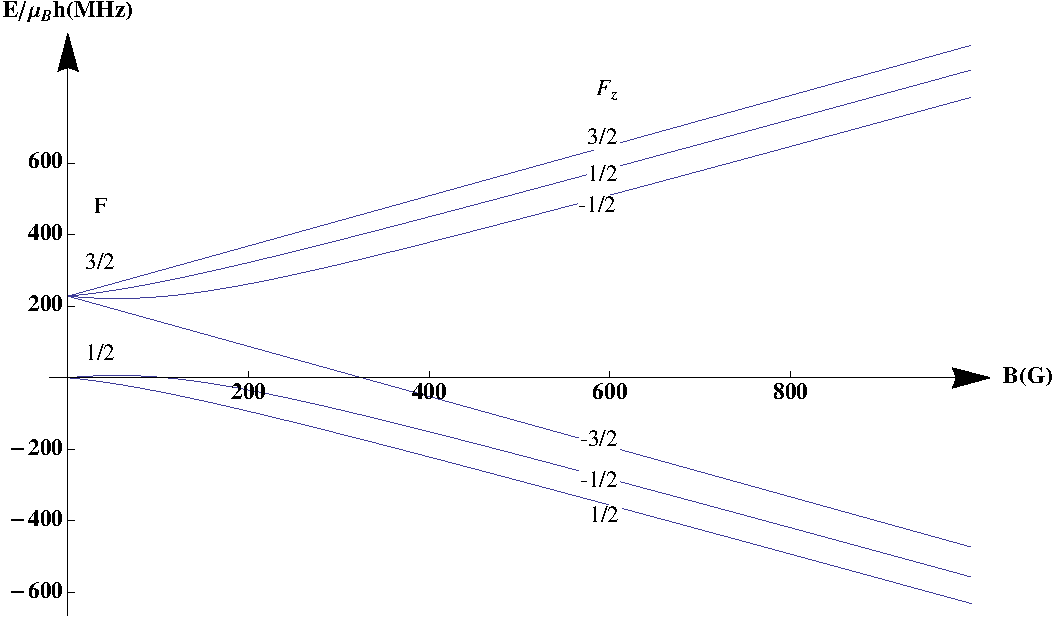
\includegraphics[width=0.8\textwidth]{hyperfineLi6}
\caption{Hyperfine structure of single \textsuperscript{6}Li atom } 
Levels are marked with $F$ and $F_{z}$ {(see Footnote \ref{foot:intro:f} in page \pageref{foot:intro:f})}
\label{fig:intro:li6}
\end{center}
\end{figure}



%\subsection{Two-body interaction}
Things will be very boring if there is only single-atom hamiltonian.  Two alkali atom interacts mostly through the overlapping of their electron clouds in the dilute setup.  Schematically the interaction can be written as 
\begin{equation}\label{eq:intro:two}
V=f(r)+g(r)\mathbf{S_{1}}\cdot\mathbf{S_{2}}
\end{equation}
The hyperfine levels that diagonalize the single atom hamiltonian is no longer eigenstates for this interaction.  In another word, if we take the direct product of hyperfine level as basis (channels) $\ket{F^{(1)},F_{z}^{(1)}}\otimes\ket{F^{(2)},F_{z}^{(2)}}$\footnote{Remember that $(F,F_{z})$ are only label, not stands for total angular momentum unless no magnetic field.\label{foot:intro:f}}, the interaction has non-diagonal term and therefore hybridizes those levels. Instead, states with definite electron spins are good basis for two-atom interaction.  In most experiments, hyperfine level is in the so-called high-field region where electron spin $S_z$ is approximately good quantum number, and therefore the original hyperfine levels serve as an good starting point as the zeroth order, i.e. channels.  When the hybridization is considered, multichannel scattering is possible.  When $g(r)$ is large enough, one channel can be deep enough and sustain a bound-state, which can lead to interesting resonance in certain parameter region.   Actually this is the essence of Feshbach resonance, and it turns out extremely useful in   cold atoms experiments.  Sec. \ref{sec:intro:twobody} briefly reviews it in two-body physics; the more involving many-body problem is then the central theme of this thesis. 

In popular experiments setup for $^{6}$Li (Fig. \ref{fig:intro:li6}), usually experiments are prepared with atoms in two lowest hyperfine levels, described by simple direct product, $\ket{F=\nth{2},F_{z}=-\nth{2}}\otimes\ket{F=\nth{2},F_{z}=+\nth{2}}$.  This is a good approximation until when two atoms are very close.  Recall that the two-atom interaction (Eq. \ref{eq:intro:two}) conserves the z-component of total angular momentum, $F_{z}^{(1)}+F_{z}^{(2)}$.  Therefore this states mixed with four other possible channels, $\ket{\nth{2},-\nth{2}}\otimes\ket{\frac{3}{2},+\nth{2}}$, $\ket{\frac{3}{2},-\nth{2}}\otimes\ket{\nth{2},+\nth{2}}$, $\ket{\frac{3}{2},+\frac{3}{2}}\otimes\ket{\frac{3}{2},-\frac{3}{2}}$, $\ket{\frac{3}{2},+\frac{1}{2}}\otimes\ket{\frac{3}{2},-\frac{1}{2}}$ (All states is labeled as $\ket{F,F_{z}}$).  There are plenty of chances for resonance, and indeed, there are several of them.  Note that close to the resonance, it is normally sufficient to consider only the one channel that is in resonance, while neglect all others.  Another important aspect is whether the two channels share one single hyperfine levels (three species) or not (four species).   Indeed the close channel in the most studied resonance close 834G is approximately $\ket{\frac{3}{2},-\nth{2}}\otimes\ket{\nth{2},+\nth{2}}$ and the resonance is a three-species one\cite{ZhangThesis,ChengRMP}. 

\section{S-wave scattering length, Bethe-Peierls boundary condition, universality, two-body density matrix\label{sec:intro:as}}
In dilute ultracold alkali gas, both the density and temperature are so low that in most case, the interaction can be characterized by a single two-body parameter, s-wave scattering length, $a_s$.  Often this is  interpreted as we can replace the real potential as a pseudo potential\cite{pethick}.  Nevertheless, an alternative interpretation about $a_s$ is more useful in this work\cite{LeggettBEC, Tan2008-1,Tan2008-2,CombescotTan}.  For short-range potential, where potential range $a_c$ is much smaller than average inter-particle distance $a_0$, it is not hard to see in the majority of the time, particles are free-like.  They only interact  when two particles are close to each other.  We can schematically divide the Hilbert space into two regions: $\mathcal{D}$, where any two particles are more than $a_c$ away from each other; and otherwise, $\mathcal{I}$ .  In the very dilute case, most physical quantities can be calculated only considering the free part, $\mathcal{D}$.  The effect of the potential on wave-function in the short-range region, $\mathcal{I}$, is to enforce the boundary condition on free part $\mathcal{D}$, $\psi(r)\xrightarrow{r\to0}\psi_{0}(r)$.  For an isometric $\psi_{0}(r)$, the lowest order in radial coordinator $r$ is $\nth{r}$.   Including the next order, a constant,  we have $\psi_{0}(r)=\nth{r}(1-\frac{r}{a_{s}})$ barring the normalization.  All these consideration gives us the simplest non-trivial boundary condition
\begin{equation}\label{eq:intro:Bethe}
\psi(r)\xrightarrow{r\to0}\nth{r}-\nth{a_s}
\end{equation}
which is also known as Bethe-Peierls boundary condition\cite{BethePeierls}.  Because of the diluteness, in the interacting region, $\mathcal{I}$, we only need to consider the two-body interaction.  Therefore, we can determine $a_{s}$ through two-body physics.  And   this simple boundary condition applies to two-body, few-body, as well as many-body context, and proves to be a very powerful tool to various problems.  

Eq. \ref{eq:intro:Bethe} coincides the zero-energy s-wave scattering wave function with very small phase-shift and that explain the name of parameter ``$a_s$''. Nevertheless,   note we did not mention anything about zero energy, where $a_{s}$ is defined in scattering theory context, and indeed this boundary condition applies generally to  any weak (positive or negative) energy solution as long as the energy involved is much lower than the energy scale in interaction region $\mathcal{I}$.  Therefore it is easy to extend it to close-to-threshold bound state.  A weak bound-state has wave function $\psi(r)=\nth{r}e^{-r/a_s}$ in $\mathcal{D}$,\footnote{The extra $\nth{r}$ factor is there for  radial wave function in 3D.} which matches Bethe-Peierls boundary condition with a positive $a_{s}$ (for  $r\ll{}a_{s}$), and we have the often cited relation for binding energy $E_{b}$.
\begin{equation}
 E_{b}=\frac{\hbar^{2}}{2ma_{s}^{2}}
\end{equation}
  This immediately clears one often confusing and counter-intuitive fact, that positive  $a_s$ corresponds to bound state.  If interpreting in the normal scattering theory, positive $a_s$  usually associates with the repulsive interaction, which obviously does not support a bound state.\footnote{This seemingly paradox can be resolved carefully within scattering theory as following. In scattering theory, the fact,  repulsive interaction leads to positive phase shift and therefore positive $a_s$, and attractive interaction leads to negative phase shift and negative $a_s$, is only true when interaction is weak, phase shift and $a_s$ is small.  At the strong interaction, where bound state is formed, phase shift changes $2\pi$; $a_s$ is large and  change sign over the threshold. }

 S-wave scattering length, $a_s$, or Eq. \ref{eq:intro:Bethe}, does not fix the normalization on the wave function. This normalization factor, turns out to be very useful.  In a dilute and low-energy system, the full system, its square is proportional to  \emph{integrated contact intensity}, $C$, defined in \cite{ Tan2008-1,Tan2008-2,CombescotTan}, besides a simple constant factor and total density.  At the limit where $a_c\to0$, $C$ and $a_s$ alone, can describe several important physical quantities, (for example internal energy).  A particular useful one for this thesis is the limit at high-momentum distribution of particles, 
 \begin{equation}
 n_k=\frac{C}{k^4}
 \end{equation}
 Note that here \emph{high-momentum} does not mean the absolutely high-momentum, it means lower than the characteristic momentum of potential $1/r_c$, but higher than any other scale, $1/a_0$,...  
 
 Indeed, if the short-range and low-energy approximation still applies, we can predict that system  does not change much from two-body, few-body to many-body at the very high-momentum ($>1/r_{c}$), where two-body wave function serves as good approximation. 
 
 In many-body physics, lots of physical observable quantities relate to one set of  quantities, density matrix, $\av{\Psi^\dg\Psi^\dg\cdots\Psi\Psi}$. In fermionic system,  one-body density matrix is often very close to the free case, although the difference can be important for various theories (such as Landau Fermi liquid theory).  Two-body density matrix is often more use with more strikingly qualitative change, especially for phenomenon involving pairing. Formally, we can decompose it into orthogonal basis
 \begin{equation}
 \av{\Psi^\dg(x_1)\Psi^\dg(x_2)\Psi(y_2)\Psi(y_1)}=\sum_nC_n\phi_n^\dg(x_1,x_2)\phi_n(y_1,y_2)
 \end{equation}     
 When one or a few $C_n$ is macroscopic, the system behaves quantum mechanically in macroscopic term.  Especially when only one term is macroscopic, system can often be interpreted as one macroscopic wave function.\cite{Leggett}  This can serves as the starting point for several phenomenon, such as BEC, BCS superconductor,...
 
Shizhong and Leggett developed independently another universality theory based on two-body density matrix \linebreak[2] \cite{shizhongUniv}, which actually takes a more general case.   They asserted that for short-range potential and low temperature, for example dilute ultracold alkali gas, the basis wave functions $\phi_n$ follows the two-body wave function at short-range. This is actually similar as Bethe-Peierls boundary condition Eq. \ref{eq:intro:Bethe}.  Instead of require the simplest form of $\psi_0$ in Eq. \eqref{eq:intro:Bethe}, they requires a more general wave-function that solves the  hamiltonian in two-body level.  And not surprisingly, many physical properties are determined by the normalization factors in boundary condition.  

In this thesis, similar idea is used along this line.  However, open-channel does not follow its two-body short-range wave-function because sensitive nature of resonance. 
 
 
 \section{Two-body Feshbach resonance\label{sec:intro:twobody}}
 As we discussed in Sec. \ref{sec:intro:as}, two-particle interaction is often approximated by a pseudo-potential characterized with s-wave scattering length $a_{s}$ in a dilute system.   The drastic  change  of $a_{s}$  via tuning energy difference (magnetic field) between two channels in Feshbach resonance gives  experimentalists the rare ability to tune the interaction strength between two particles.  And it is extremely useful in the study of BEC-BCS crossover where the interaction varies from weak to strong.  
 
Here we briefly review the Feshbach resonance in two-body system.   As discussed in Sec. \ref{sec:intro:one}, for isolated single atom, hyperfine level is the eigenstate.  However, when two atoms interacts, most of interaction comes from interaction of electrons while nucleons interacts very little.  Therefore, hyperfine levels is no longer true eigenstates of the two-body system and two hyperfine.  Nevertheless, hyperfine level serves a good approximated quantum number and levels are still labelled with it. Furthermore, we take ``channels'' as pair of hyperfine indices, they are in general different in interaction strength and are decoupled in the lowest order.  In magnetic field, different channels differ in energy mostly due to the Zeeman energy of electronic spin as electronic magnetic moment is much larger than nuclear magnetic moment.  This energy difference is easy to tune via magnetic field.  

When mixture between channels are taken into consideration, the simple single-channel scattering becomes multi-channel scattering.  Especially, when the one channel's threshold is close to a bound-state in the other channel when considered isolated, the scattering property in this channel is dramatically altered,  phase shift can changes $2\pi$ and s-wave scattering length $a_{s}$ changes to infinity and jumps to the infinity in opposite sign.  This is essentially what happens in Feshbach resonance, which was studied by Fano\cite{Fano} and Feshbach \cite{nuclear}  in nuclear and atom physics 1960s.  Here we  mostly follow treatment in \cite{Leggett} (with some different symbols to comply with the rest of this thesis). 
\footnote{Here I list a few main different symbols, with the symbols from \cite{Leggett} in parenthesis.  $U$ ($=-V$): open-channel interaction; $V$ ($=-V_{c}$): close-channel interaction; $Y$ (=-$g\cdot{}f$): inter-channel coupling; $E_{b}$ ($=\epsilon_{0}$):binding energy of close-channel bound state; $a_{c}$ ($=r_{0}$): range of potential; $\eta$ ($=\epsilon_0+\tilde\delta$) the Zeeman energy difference between two channels; $\mathcal{K}$ ($=\kappa$) see Eq.\ref{eq:intro:kappa}.}

The two-channel hamiltonian can be written as ($2\times2$ matrix for  (open,close) ``spinor'')
\begin{equation}
\hat{H}(r)=
\begin{pmatrix}
-\frac{\hbar^{2}}{2m_{r}}\nabla^{2}-U(r)&,&-Y(r)\\
-\frac{\hbar^{2}}{2m_{r}}\nabla^{2}+\eta-V(r)&,&-Y(r)
\end{pmatrix}
\end{equation}
where energy zero is counted from that of the open channel at infinite separation. $\eta$ is the absolute difference in Zeeman energy of two channels.  All the interactions are short-range.  For a s-wave solution we have 
\begin{equation}
\psi(r)=\nth{r}\mtrx{\chi(r)\\\chi_{c}(r)}
\end{equation}
Now we can write down the time-independent \sch equation in radial direction for the scattering state:
\begin{align}
-\frac{\hbar^{2}}{2m_{r}}\chi''-U\chi-Y\chi_c&=E\chi\label{eq:intro:open}\\
-\frac{\hbar^{2}}{2m_{r}}\chi_c''+\eta\chi_c-V\chi_c-Y\chi&=E\chi_c
\end{align}
We expand close-channel wave function $\chi_{c}$ over the eigenstates of close-channel hamiltonian, $\phi_{i}$, 
\begin{equation}
-\frac{\hbar^{2}}{2m_{r}}\phi_{i}''-V \phi_{i}=-E_{b}^{(i)}\phi_{i}
\end{equation}
Here we assume the energy difference between levels are larger than other energy scale and keeps only the one in resonance, $\phi_{0}$.  Na\"{i}vely speaking, the resonance happens at the point where the close-channel bound state level is exactly at the threshold of open-channel.  Therefore we introduce the relative detuning, $\tilde\delta=\eta-E_{b}$ It is not hard to find
\begin{equation}
\chi_{c}=\frac{\phi_{0}}{E-\tilde\delta}\int{dr'}\,\phi_{0}^{*}(r')Y(r')\chi\br{r'}
\end{equation}
Note that here $\phi_{0}$ is normalized (for radial component).  Put this back to \sch equation of open-channel component $\chi$ (Eq. \ref{eq:intro:open}), 
\begin{equation}\label{eq:intro:chi}
\br{-\frac{\hbar^{2}}{2m_{r}}\frac{d^{2}}{dr^{2}}-U-E}\chi+\frac{1}{E-\tilde\delta}\int_{0}^{\infty}K(r\,r')\chi(r')dr'=0
\end{equation}
where kernel $K(r\,r')$ is
\begin{equation}
K(r\,r')\equiv\phi_{0}(r)\phi_{0}(r')Y(r')Y(r)\equiv{}K(r'\,r)
\end{equation}
Compare this with open-channel scattering \sch equation without coupling to close-channel
\begin{equation}\label{eq:intro:chi0}
\br{-\frac{\hbar^{2}}{2m_{r}}\frac{d^{2}}{dr^{2}}-U-E}\chi_{0}=0
\end{equation}
Note that $\chi_{0}(r)\rightarrow0$ as $r\rightarrow0$ and $\chi_{0}(r)\rightarrow\text{const}(1-r/a_{bg})$ for $r\rightarrow\infty$\footnote{Note that we are dealing with the internal wave function $\chi_{0}$ here (in region $\mathcal{I}$) instead of the external wave function as in Sec. \ref{sec:intro:as}, therefore, the boundary condition for $r\rightarrow0$ there actually corresponds boundary condition $r\rightarrow\infty$ here.}  Now multiply Eq. \ref{eq:intro:chi} with $\chi_{0}$ and Eq. \ref{eq:intro:chi0} with $\chi$, subtract them, and use Green's theorem, we find 
\begin{equation}
\chi_{0}(r_{c})\chi'(r_{c})-\chi_{0}'(r_{c})\chi(r_{c})+\frac{2m_{r}E}{\hbar^{2}}\int_{0}^{r_{c}}dr\chi_{0}(r)\chi(r)
=\frac{2m_{r}/\hbar^{2}}{E-\tilde\delta}\int_{0}^{r_{c}}dr\int_{0}^{r_{c}}dr'\chi_{0}(r)K(rr')\chi(r')
\end{equation}
Here $r_{c}$ is a  distance much larger than potential range, and we can use the boundary condition by let $r\rightarrow\infty$, $\chi_{0}(r)\rightarrow\text{const}(1-r/a_{bg})$, $\chi(r)\rightarrow\text{const}(1-r/a_{s})$.  The R.H.S approaches a constant for a short-range interaction $Y(r)$ and therefore $K(rr')$.  For scattering solution at  $E=0$, we have 
\begin{equation}
\nth{a_{s}}-\nth{a_{bg}}=\frac{2m_{r}/\hbar^{2}}{\tilde\delta}\int_{0}^{\infty}dr\int_{0}^{\infty}dr'\chi_{0}(r)K(rr')\chi(r')
\end{equation}
Contrary to na\"ive intuition, $a_{s}$ does not diverge at the point $\tilde\delta=0$ because of the original interaction in open-channel, $a_{bg}$.  We can define a quantity $\mathcal{K}$, the detuning where $a_{s}$ diverges, by the implicit equation ($\mathcal{K}$ shows up in R.H.S as well)
\begin{equation}\label{eq:intro:kappa}
\mathcal{K}\equiv-\frac{2m_{r}a_{bg}}{\hbar^{2}}\int_{0}^{\infty}{dr}\int_{0}^{\infty}dr'\chi_{0}(r)K(rr')\chi_{\tilde\delta=\mathcal{K}}(r')
\end{equation}
And if we define the ``real detuning'' $\delta\equiv\tilde\delta-\mathcal{K}$, we have 
\begin{equation}
a_{s}(\delta)=a_{bg}\br{1+\frac{\kappa}{\delta}}
\end{equation}
Comparing this with the empirical formula of Feshbach resonance
\begin{equation}
a_{s}(B)=a_{bg}\br{1+\frac{\Delta{B}}{B-B_{0}}}
\end{equation}
We see that $\Delta{B}=\mathcal{K}(\partial\delta/\partial{B})^{-1}$, and $B_{0}$ is the real resonance position.  Here $\partial\delta/\partial{B}$ is the magnetic momentum difference between two channels.  

Next we consider the bound state where $E<0$, define
\begin{equation}\label{eq:intro:ab}
a_{b}(E)\equiv\frac{\hbar}{(2m_{r}\abs{E})^{1/2}}
\end{equation}
Note that $a_{b}(E)$ is not identified as $a_{s}$ a priori.  Here we only study the bound state close to threshold with binding energy much smaller than the binding energy of close-channel bound state $\phi_{0}$, $\abs{E}\ll\epsilon_{0}$, and therefore $a_{b}\ll{a_{c}}$.  Outside the range of potential $a_{c}$,  the wave function is proportional to $e^{-r/a_{b}}$. For $a_{c}\ll{}r\ll{}a_{b}$, it is approximately $1-\frac{r}{a_{b}}$, just as the s-wave scattering wave function.  We can go through the similar procedure as previous, and it is not hard to find (We assume the short-range part of wave function $chi$ does not change much and therefore $\mathcal{K}$ stays relatively constant)
\begin{equation}
\frac{a_{bg}}{a_{b}}-1=\frac{-\mathcal{K}}{\delta+\mathcal{K}-E}
\end{equation}
Provided both $\delta$ and $\abs{E}$ are much smaller than $\mathcal{K}$, this leads to 
\begin{equation}\label{eq:intro:abKE}
a_{b}=\frac{\mathcal{K}}{\delta-E}
\end{equation}
It is not hard to see that $a_{b}$ coincides with s-wave scattering length $a_{s}$ when $\abs{E}\ll\abs{\delta}$, and therefore we will use them interchangeably afterward. This is actually an example our discussion about Bethe-Peierls boundary condition in Sec. \ref{sec:intro:as}.  Using Eqs. \ref{eq:intro:ab} and \ref{eq:intro:abKE}, it is easy to obtain an equation for $E$
\begin{equation}
(\abs{E}+\delta)^{2}-2\delta_{c}\abs{E}=0
\end{equation}
where $\delta_{c}$ is defined as 
\begin{equation}
\delta_{c}\equiv\frac{\mathcal{K}^{2}}{\hbar^{2}/m_{r}a_{bg}^{2}}
\end{equation}
And the solution is  (for $\delta<0$)
\begin{equation}
\abs{E}=\delta_{c}-\delta-\sqrt{\delta_{c}^{2}-2\delta\delta_{c}}
\end{equation}
Furthermore, we can calculate the ``relative weight'' (probability) of close-channel 
\begin{equation}
\lambda=\br{\frac{1}{E-\tilde\delta}}^{2}\abs{\int{}dr'\phi_{0}(r')Y(r')\xi_{n}(r')}^{2}
\end{equation}
where $\xi_{n}(r)$ is the normalized open-channel bound-state component.  Comparing this with Eq. \ref{eq:intro:kappa}, assume the short-range part of $\chi_{n}(r)$ does not differ from $\chi_{o}(r)$ much, we can find 
\begin{equation}
\lambda=\nth{(E-\tilde\delta)^{2}}\frac{\hbar^{2}}{2m_{r}a_{bg}}\mathcal{K}a_{b}^{-1}
\end{equation}
For $\abs{\delta}\lesssim\delta_{c}\ll\mathcal{K}$, $E-\tilde\delta\approx\mathcal{K}$ and we have 
\begin{equation}
\lambda=\frac{\hbar^{2}}{2m_{r}a_{bg}}\nth{(\mathcal{K}a_{b})}=\br{\frac{\abs{E}}{2\delta_{c}}}^{1/2}
\end{equation}
Now we can see that  $\delta_{c}$ is a ``characteristic'' energy scale. When $\abs{\delta}\gg\delta_{c}$, $E\approx\delta$, this simply means that when the negative detuning is large, most weight is in close-channel, and the real mixed bound state is a close-channel bound state ($\phi_{0}$) dressed with little open-channel component and therefore the binding energy is roughly equal that of $\phi_{0}$.  On the contrary, when $\abs{\delta}\ll\delta_{c}$, $\abs{E}\approx-\delta^{2}/\delta_{c}\ll\delta$,  and close-channel weight is much smaller than that of open-channel, the real bound-state is more or less a open-channel affair with little dress-up from close-channel.  % It is not hard to  estimate $\delta_{c}$. 

In the many-body physics, another important energy scale comes into play, Fermi energy, $E_{F}$.  When it is much smaller than $\delta_{c}$, i.e. \emph{broad resonance},  close-channel has only negligible weight close to resonance, where we are mostly interested in. In such situation, it is a good approximation to take Feshbach resonance as only a knob to tweak the interaction over open-channel there.  On the contrary, when $E_{F}$ is close even larger than $\delta_{c}$, i.e. \emph{narrow resonance}, close-channel weight can be  significant around resonance, therefore requires to be explicitly taken into many-body framework.  










\section{Single-channel BEC-BCS crossover}
In this section, we briefly review the BEC-BCS crossover in single channel.   The interaction strength is tuned along the crossover region.  This applies directly to the broad-resonance, where the close-channel weight is negligible and serves only to modify the effective strength in open-channel.  We  mostly follow treatment in \cite{RanderiaBEC, Randeria1997, Randeria2008}.
%\subsection{Path integral for one channels}
% !TeX root =thesis.tex
%\subsection{Path integral approach for single channel\label{sec:pathInt}}
\label{sec:pathInt}
Randeria and the company has studied this problem with path integral and it is proved to be a rather nice tool for the problem due to its flexibility and readiness for extension to higher order fluctuation.  

We start with an attractive $\delta$-potential in real space.  This is not equivalent to the l reduced pairing potential as in original BCS work.  However, reduced paring potential only couples  particles of the opposite momentum and does not support simple form of Hubbard-Stratonovich transformation, which is essential to solve the problem in path integral formulation.  
\begin{equation}
\hat{H}-\mu\hat{N}=\sum_{\sigma}\int{d^{d}r}c^{\dagger}_{\sigma}(\vr)\br{-\nth{2m}\nabla^{2}-\mu}c^{}_{\sigma}(\vr)-g\int{d^{d}r}c^{\dagger}_{\uparrow}(\vr)c^{\dagger}_{\downarrow}(\vr)c^{}_{\downarrow}(\vr)c^{}_{\uparrow}(\vr)
\end{equation}
 We can write down the action for the quantum partition function $\mathcal{Z}=\int{D(\bar\psi,\psi)\exp\br{-S[\bar\psi,\psi]}}$
\begin{equation}
S[\bar\psi,\psi]=\int^{\beta}_{0}d\tau\int{d^{d}r}\mbr{\sum_{\sigma}\bar\psi_{\sigma}(\vr,\tau)\br{\partial_{\tau}-\nth{2m}\nabla^{2}-\mu}\psi_{\sigma}(\vr,\tau)-g\bar\psi_{\uparrow}(\vr,\tau)\bar\psi_{\downarrow}(\vr,\tau)\psi^{}_{\downarrow}(\vr,\tau)\psi^{}_{\uparrow}(\vr,\tau)}
\end{equation}
We try to solve this system by introduce Hubbard-Stratonovich transformation.   Introduce a bosonic field $\Delta(\vr,\tau)$ coupled with Cooper channel $\psi(\vr,\tau)\psi(\vr,\tau)$. %Here we follow the normal notation from path integral, $r$ is four tempo-space coordinator.  
We write down first the Gaussian integral of $\Delta$
\begin{equation}
1=\int{D(\bar\Delta,\Delta)}\exp\br{-\nth{g}\int{d\tau{d}^{d}r}\bar\Delta\Delta}
\end{equation}
Note that we absorb the extra constant of integration into the measure of $D(\bar\Delta,\Delta)$.
And with a shift of $\Delta(\vr,\tau)\rightarrow\Delta(\vr,\tau)-g\psi(\vr,\tau)\psi(\vr,\tau)$, we have 
\footnote{$\int{D(\bar\Delta,\Delta)}\cdot1$ is only a constant factor on partition function $\mathcal{Z}$ and has no effect on real physical quantity, therefore, we can take it as 1, (equivalently divide the $\mathcal{Z}$ by a constant)}
\begin{equation}
\exp\br{g\int{d\tau{}d^{d}r}\psi_{\uparrow}\bar\psi_{\downarrow}\psi_{\downarrow}\psi_{\uparrow}}=
\int{D(\bar\Delta,\Delta)}\exp\bbr{-\int{d\tau{d^{d}r}}\mbr{\nth{g}\abs{\Delta}^{2}-\br{\bar\Delta\psi_{\downarrow}\psi_{\uparrow}+\Delta\bar\psi_{\uparrow}\bar\psi_{\downarrow}}}}
\end{equation}
Now the interaction term can be replaced.
\begin{equation*}
\mathcal{Z}=\int{D(\bar\psi,\psi)\int{D(\bar\Delta,\Delta)}\exp\bbr{-\int{d\tau{d^{d}r}}\mbr{\sum_{\sigma}\bar\psi_{\sigma}\br{\partial_{\tau}-\nth{2m}\nabla^{2}-\mu}\psi_{\sigma}+\nth{g}\abs{\Delta}^{2}-\br{\bar\Delta\psi_{\downarrow}\psi_{\uparrow}+\Delta\bar\psi_{\uparrow}\bar\psi_{\downarrow}}}}}
\end{equation*}
This form is bilinear to $\psi$, and we can rewrite it into a nicer form in Nambu spinor representation
\begin{equation}
\bar\Psi=\begin{pmatrix}\bar{\psi}_{\uparrow}&\psi_{\downarrow}\end{pmatrix}\text{,  }\qquad
\Psi=\begin{pmatrix}{\psi}_{\uparrow}\\\bar\psi_{\downarrow}\end{pmatrix}
\end{equation}
\begin{equation}
\mathcal{Z}=\int{D(\bar\psi,\psi)}\int{D(\bar\Delta,\Delta)}\exp
	\bbr{-\int{d\tau{d^{d}r}}\mbr{\nth{g}\abs{\Delta}^{2}-\bar\Psi \nG\Psi}}
\end{equation}
where 
\begin{equation}\label{eq:pathInt:nG}
\nG=\begin{pmatrix}
[\hat{G}_{0}^{(p)}]^{-1}&\Delta\\\bar\Delta&[\hat{G}_{0}^{(h)}]^{-1}
\end{pmatrix}
\end{equation}
is known as Gor'kov Green function, and $[\hat{G}_{0}^{(p)}]^{-1}=-\partial_{\tau}+\nth{2m}\nabla^{2}+\mu$, and $[\hat{G}_{0}^{(h)}]^{-1}=-\partial_{\tau}-\nth{2m}\nabla^{2}-\mu$ represent the non-interacting Green functions of the particle and hole respectively. Now $\Psi$ can be integrated out formally and partition function then only depends on bosonic field $\Delta$.
\begin{equation}\label{eq:pathInt:DeltaPF}
\mathcal{Z}=\int{D(\bar\Delta,\Delta)}\exp
	\bbr{-\mbr{\br{\int{d\tau{d^{d}r}}\nth{g}{\bar\Delta\Delta}}-\ln\det\nG}}
\end{equation}
And action is
\begin{equation}\label{eq:pathInt:DeltaAction}
S[\bar\Delta,\Delta]=
	{\mbr{\br{\int{d\tau{d^{d}r}}\nth{g}{\bar\Delta\Delta}}-\ln\det\nG}}
\end{equation}
Note that $\ln\det\nG$ goes through both the normal space and $2\times2$ Nambu spinor space.  

\subsection{Mean Field Result\label{sec:pathInt:meanfield}}
The saddle point equation of Eq. (\ref{eq:pathInt:DeltaPF}) gives the mean-field result of the system.  First we need to find the derivative of $\ln\det\nG$.  We notice the identity
\begin{equation}
\ln\det\hat{A}=\tr\ln\hat{A}
\end{equation}
and differential rule of a function like $\tr\ln$
\begin{equation}\label{eq:pathInt:diffTr}
\frac{\delta}{\delta\phi_q}\tr\ln(\nG)=\tr(\hat{\mathcal{G}}\frac{\delta}{\delta\phi_q}\nG)
\end{equation}
The saddle equation of Eq. (\ref{eq:pathInt:DeltaPF}) (differential with respect to $\Delta$) is
\begin{equation}
\nth{g}\bar{\Delta}(\vr,\tau)-\tr\mbr{\hat{\mathcal{G}}(\vr,\tau,\vr,\tau)\begin{pmatrix}0&1\\0&0\end{pmatrix}}=0
\end{equation}
Here this matrix is in the Nambu Spinor space.  If we seek a tempo-spacial homogeneous solution of $\Delta_0$, we can find the Nambu Green function from Eq. (\ref{eq:pathInt:nG}) in momentum space
\begin{equation}\label{eq:pathInt:G0}
G_0(p)=\nth{(i\omega_n)^2-E_\vp^2}
\begin{pmatrix}
	i\omega_n+\xi_\vp&-\Delta_0\\
	-\bar{\Delta}_0&i\omega_n-\xi_\vp
\end{pmatrix}
\end{equation}
Here $\omega_n$ is Matsubara frequency of Fermions.  $\xi_{\vk}=\epsilon_{\vk}-\mu$, $\epsilon_{\vk}=\vk^{2}/2m$,  $E_\vp=\sqrt{\xi_\vp^2+\abs{\Delta_0}^2}$.  And the saddle point equation can be rewritten as 
\begin{equation}
\nth{g}\bar{\Delta}_0=\frac{T}{L^d}\sum_{\vp,n}\frac{\bar\Delta_0}{\omega_n^2+E_\vp^2}
\end{equation}
The summation of Matsubara frequency can be evaluated and we find 
\begin{equation}
\nth{g}=\nth{L^d}\sum_{\vp}\frac{1-2n_f(E_p)}{2E_p}=\nth{L^d}\sum_{\vp}\frac{\tanh{(E_p/2T)}}{2E_p}
\label{eq:pathInt:gap}
\end{equation}
where $n_f(\epsilon)$ is the fermi distribution function.  This is exactly the gap equation obtained from other methods as well.  On the other hand, $\nG$ in Eq. (\ref{eq:pathInt:nG})  is the inverse of fermion-fermion correlation of $\Psi$.  In mean field, $G_{0}$ as Eq. (\ref{eq:pathInt:G0}) can be diagnosed in momentum space with a canonical (Bogoliubov) transformation.  Nevertheless, poles is where  $\omega^2-E_\vp^2=0$ (with a analytic continue of $i\omega_{n}\rightarrow\omega+0^{+}$) as we can see from  Eq. (\ref{eq:pathInt:G0}) and therefore the spectrum of fermionic excitation is $\pm{}E_{p}$.  

Summand in Eq. \ref{eq:pathInt:gap} does not decreases fast enough in 3D and the summation does not converges.  This is because our assumption of contact interaction breaks down when reaching real potential range $a_{c}$, i.e., the summation of momentum is capped at some high momentum $\Lambda$ related to $1/a_{c}$.  Notice that in 3-D, we have a relation that connect the bare potential $g$ to more physically observable s-wave scattering length $a_{s}$
\begin{equation}\label{eq:pathInt:as}
\frac{m}{4\pi{}a_{s}}=-\nth{g}+\sum_{k<\Lambda}\nth{2\epsilon_{\vk}}
\end{equation}
We can renormalize Eq. \ref{eq:pathInt:gap} with this relation
\begin{equation}
-\frac{m}{4\pi{}a_{s}}=\sum_{\vk}\mbr{\frac{\tanh{(E_k/2T)}}{2E_k}-\nth{2\epsilon_{\vk}}}
\end{equation}
Now the gap equation has proper decay in high momentum and no artificial cutoff is necessary.  There are two unknown parameters, $\mu$ and $\Delta$,  in the equation.  We need another equation in order to pin them down. To compliment the gap equation, we can introduce the number equation, $n=-\partial\Omega/\partial\mu$. At the saddle point, the thermodynamic potential is $\Omega_{0}=S[\Delta_{0}]/\beta$, and we have number equation
\begin{equation*}
n=-\nth{\beta}\tr\br{{G_{0}\pdiff{G_{0}^{-1}}{\mu}}}
\end{equation*}
similarly the summation over the Mastubara frequency can be evaluated and we have equation
\begin{equation}
n=\nth{L^{d}}\sum_{\vk}\mbr{1-\frac{\epsilon_{\vk}}{E_{\vk}}\tanh{(\frac{E_{\vk}}{2T})}}
\end{equation}

\subsection{Gaussian fluctuation and collective mode}\label{sec:collective1}
Once the mean field value is obtained, we can expand partition function Eq. (\ref{eq:pathInt:DeltaPF}) around it ($\Delta(\vr,\tau)=\Delta_{0}+\eta(\vr,\tau)$). The linear order of  expansion is zero because $\Delta_{0}$ is the saddle point.  The next order gives us the bilinear terms on $\eta$, i.e., correlation of bosonic field $\Delta$ (four-fermion correlation).  Note that here the hamiltonian only has an extreme-short-range ($\delta$) potential, therefore it cannot cover the situation of charged system where long-range Columnb interaction cannot be neglected.  We will discuss this later.  Nevertheless, it is conceivable that a more realistic short-range potential only renormalizes some parameters in the following calculation while leaves the qualitative result unmodified.  

Notice that we can expand the second term in Eq. \ref{eq:pathInt:DeltaPF} for $\hat{G}{}^{-1}=\hat{G}_{0}^{-1}+\hat{K}$
\begin{equation}\label{eq:pathInt:expand}
\tr\ln \hat{G}^{-1}=\tr\ln\hat{G_{0}}^{-1}+\tr(\hat{G_{0}}\hat{K})-\nth{2}\tr(\hat{G_{0}}\hat{K}\hat{G_{0}}\hat{K})+\cdots
\end{equation}
In our case,
\begin{equation}
\hat{K}=\begin{pmatrix}
0&\eta\\
\eta^{*}&0
\end{pmatrix}
\end{equation}
Here the linear terms of $\hat{K}$ or $\eta$ ($\eta^{*}$) are zero as the saddle point condition.  So to the second order, the action is 
\begin{equation}\label{eq:pathInt:DeltaActionGaussian}
S[\Delta_{0},\eta,\eta^{*}]=S[\Delta_{0}]+
	\nth{2g}\tr(\hat{K}\hat{K})+\nth{2}\tr(\hat{G_{0}}\hat{K}\hat{G_{0}}\hat{K})
\end{equation}
Write the last term into the momentum representation
\begin{equation}
\tr(\hat{G_{0}}\hat{K}\hat{G_{0}}\hat{K})=\sum_{q,p}\Tr\br{G_{0}({p})K_{q}G_{0}{}({p-q})K_{-q}}
\end{equation}
Notice that the second ``$\Tr$'' and following ``$\Tr$'' in this section only runs in Nambu spinor space and $q={(\vq,q_{l})}$, $p=(\vp,p_{n})$ are all four momentum, where $q_{l}$ is bosonic Matsubara frequency while $p_{n}$ is fermionic Matsubara frequency.
\begin{equation}
K_{q}=\begin{pmatrix}
0&\eta_{q}\\
\eta^{*}_{-q}&0
\end{pmatrix}
\end{equation}
If we introduce the a new vector 
\begin{equation}
\eta{(q)}=\begin{pmatrix}\eta_{q}\\\eta^{*}_{-q}\end{pmatrix}\qquad
\eta^{\dg}{(q)}=\begin{pmatrix}\eta^{*}_{q}&\eta_{-q}\end{pmatrix}
\end{equation}
the action can be rewritten into a more compact form
\begin{equation}
S[\Delta_{0},\eta,\eta^{*}]=S[\Delta_{0}]+\nth{2}\sum_{q}\Tr\mbr{\eta^{\dg}(q)\mathbf{M(q)}\eta(q)}
\end{equation}
Notice that we can always choose a real $\Delta_{0}$ and therefore $G_{0}{\ _{12}}(p)=G_{0}{\ _{21}}(p)$, we have 
\begin{equation}
\mathbf{M(q)}=
\begin{pmatrix}
\nth{g}+\sum_{p}G_{0}{\ }_{11}(p)G_{0}{\ }_{22}(p-q)&\sum_{p}G_{0}{\ }_{12}(p)G_{0}{\ }_{12}(p-q)\\
\sum_{p}G_{0}{\ }_{12}(p)G_{0}{\ }_{12}(p-q)&\nth{g}+\sum_{p}G_{0}{\ }_{11}(p-q)G_{0}{\ }_{22}(p)
\end{pmatrix}
\end{equation}
The summation over (fermionic) Matsubara frequency of $p_{n}$ can be carried out at zero temperature
\footnote{\label{foot:intro:sum}The summation of Matsubara frequency of function $h(i\omega_{n})$ is carried out by the normal method to multiplying $h(z)$ with fermi distribution function $n_{F}(z)$, and then find all residues with a contour over infinity.  However, due to zero temperature, the  $n_{F}(z)$ only nonzero at the negative singular points of $h(z)$, $-E_{\vk}$ in our case.  (The other singular point $E_{\vk}$ gives $n_{F}(E_{\vk})=0$ for zero temperature.}
\begin{equation}
\begin{split}
M_{11}(q)&=M_{22}(-q)\\
	&=\nth{g}+\sum_{\vp{,}p_{n}}G_{0}{\ }_{11}(p)G_{0}{\ }_{22}(p-q)\\
	&=\nth{g}+\sum_{\vp}\br{\frac{u^{2}u'^{2}}{iq_{l}-E-E'}-\frac{v^{2}v'^{2}}{iq_{l}+E+E'}}
\end{split}
\end{equation}
\begin{equation}
\begin{split}
M_{12}(q)&=M_{21}(q)\\
	&=\sum_{\vp{,}p_{n}}G_{0}{\ }_{12}(p)G_{0}{\ }_{12}(p-q)\\
	&=\sum_{\vp}uvu'v'\br{\nth{iq_{l}+E+E'}-\nth{iq_{l}-E-E'}}
\end{split}
\end{equation}
where $u=u_{\vp}$, $v=v_{\vp}$, $E=E_{\vp}$ and $u'=u_{\vp-\vq}$, $v'=v_{\vk-\vq}$, $E'=E_{\vk-\vq}$.  $u$, $v$, $E$ are as defined usually in BCS literature. 
\begin{equation}
v_{\vk}^{2}=1-u_{\vk}^{2}=\nth{2}\br{1-\frac{\xi_{\vk}}{E_{\vk}}}
\end{equation}
 The $G^{(M)}=\mathbf{M}^{-1}$ is the correlation function of $\eta$ (or $\Delta$) and its poles give the spectrum of collective mode as every  $\eta_{q}$ (or $\Delta_{q}$) involves many fermions moving in a coherent manner.  So the spectrum of collective modes can be determined by $\det{M(\omega,\vq)}=0$ after we analytically continue for the frequency $iq_{l}\rightarrow\omega+i0^{+}$.  
 
For low energy modes, where $\omega,\,\abs{\vq}^{2}\ll\min\bbr{E_{\vk}}$ both are much smaller than $\Delta_{0}$, we can expand $M$ with $\omega$ and $\vq$.  


\subsection{Alternative in inverting green function\label{sec:diagonalizeGreen1}}
In the above section, we have inversion of Gorkov green function Eq. (\ref{eq:pathInt:nG}) and it can be invert easily as Eq. (\ref{eq:pathInt:G0}).   Alternatively, we can use a different approach which proves to be more convenient in two-channel problem.  First, we diagonalize $\nG$ with unitary transformation $T$, in momentum space
\begin{equation}
\nG=\mtrx{i\omega_{n}-\xi_{k}&\Delta\\\bar\Delta&i\omega_{n}+\xi_{k}}=T^{\dg}BT
\end{equation}
It is easy to show that such $T$ and $B$ satisfing above equation are
\begin{equation}
T=\mtrx{u_{k}&v_{k}\\-v_{k}^{*}&u_{k}}\qquad{}B=\mtrx{i\omega_{n}+E_{k}&0\\0&i\omega_{n}-E_{k}}
\end{equation}
where $u_{k}^{2}(v_{k}^{2})=\nth{2}(1\pm\xi_{k}/E_{k})$ and $E_{k}$ are conventionally defined quantities in BCS theory.   Actually, this transformation is nothing but Bogoliubov canonical transformation, and $B$ matrix simply describes spectrum of fermionic quasi-particles.  Now it is easy to invert $\nG$
\begin{equation}
G=T^{\dg}B^{-1}T
\end{equation}
Green's function $G$ takes a more conventional form $A/(i\omega_{n}-e_{k})$ without any dependency on frequency in nominator as Eq. (\ref{eq:pathInt:G0}). Matsubara frequency summation over $G_{0}(k)$ in mean-field and $G_{0}(k)G_{0}(k+q)$ in Gaussian order are then fairly straight-forward as in text-book.  




\begin{subappendices}
\section{Wave function for short-range potential}\label{sec:pathInt2:short-range}
Here we discuss some possible generalization on the wave function for short-range potential.  This topic has been studied by Shizhong Zhang \cite{shizhongUniv}. We will use some similar ideas.  Outside the range $r_{c}$ of a short-range potential,  atom is free and  \sch equation is very simple.
\begin{equation}
-\frac{\hbar^{2}}{2m}\nabla^{2}\psi=E\psi
\end{equation}
The equation has a simple solution for s-wave, $\psi=A{e^{-\kappa{r}}}/{r}$ ($\kappa$ is imaginary for scattering state), here normalization $A$ is determined  by connecting it with the short-range part of the wave function, $\varphi_0$. 

Let us discuss the bound-state first, $\kappa>0$.  In the momentum space, there is also a universal behavior at low-momentum, where $kr_{c}\ll1$.   
\begin{equation*}
\psi_{k}=\nth{(2\pi)^{3/2}}\int{d\vr}(\varphi_{0}+A\frac{e^{-\kappa{r}}}{r})e^{-i\vk\cdot\vr}
\end{equation*}
The first part for $\varphi_{0}$ has very little $k$ dependence and the second terms give
\begin{equation*}
\psi_{k}=\varphi_{0\,k}+\nth{(2\pi)^{3/2}}\int{d\vr}(A\frac{e^{-\kappa{r}}}{r})e^{-i\vk\cdot\vr}=\varphi_{0\,k}-(\frac{2}{\pi})^{1/2}A\nth{k^{2}+\kappa^{2}}
\end{equation*}

Furthermore, if the bound-state is the one close to threshold, the most weight is outside $r_{c}$, we can neglect the first term and we have universal behavior at low-momentum while the normalization is determined in two-body problem.   When considering many-body physics, in the really low momentum, (at order of Fermi energy or below), wave function  is modified, but in the medium momentum, (still much smaller than $1/r_{c}$), this universal behavior is preserved.  The number distribution of particle in such momentum, $k_{F}\ll{k}\ll{1/r_{c}}$, is $1/k^{4}$. This is actually the ``high-momentum'' (medium here) behavior ($C/k^{4}$) described in Tan's work about universality\cite{Tan2008-1,Tan2008-2}. 

On the other hand, at very high momentum ($k\gg1/r_{c}$), the second term in the above is very small.  This is because the smooth tail part of the wave function contributes little in high-oscillation.  The high-frequency Fourier component is solely determined by the wave function within the potential range.   This can be extend beyond two-body wave function to two-body correlation as long as the long-wave-length part is smooth.  In all cases, two-body, or many-body, very high-frequency of two-body correlation follows the two-body wave function.  

\end{subappendices}

